\documentclass[conference]{IEEEtran}
\IEEEoverridecommandlockouts
% The preceding line is only needed to identify funding in the first footnote. If that is unneeded, please comment it out.
\usepackage{cite}
\usepackage{amsmath,amssymb,amsfonts}
\usepackage{algorithmic}
\usepackage{graphicx}
\usepackage{textcomp}
\usepackage{xcolor}
\usepackage{floatrow}
\newfloatcommand{capbtabbox}{table}[][\FBwidth]
\usepackage{blindtext}
\usepackage{subfig}
\usepackage{hyperref}

\def\BibTeX{{\rm B\kern-.05em{\sc i\kern-.025em b}\kern-.08em
    T\kern-.1667em\lower.7ex\hbox{E}\kern-.125emX}}
\begin{document}

\title{FORENSIC ANALYSIS OF ANDROID BASED SPY APPLICATIONS}

\author{
\IEEEauthorblockN{Brennon Sullivan}
\IEEEauthorblockA{\textit{SHSU Computer Science}}}


\maketitle

\begin{abstract}
Smartphones with Google’s Android operating system are becoming more and more popular
each year, and with this increased user base, comes increased opportunities to collect more of
these users’ private data. There have been several instances of malware being made available
via the Google Play Store, which is one of the predominant means for users to download
applications. One effective way of collecting users’ private data is by using Android Spyware.
In this paper, a forensic analysis of a malicious Android spyware application was conducted and
present my findings. I also highlight what information the application accesses and what
it does with that information. I then provide my findings on how Google’s Play Protect
service handles this spyware application. Lastly, I offer a simple framework that forensic
investigators can follow for performing mobile application analysis.
\end{abstract}

\begin{IEEEkeywords}
Android, Malware, Mobile Forensics, Mobile Security, Spyware Analysis, Play Protect.
\end{IEEEkeywords}

\section{Introduction}
The Android Operating System (OS) is the most used mobile OS in the world, accounting for 76.61\% of the global market share. This makes it an ideal target for cybercriminals who make their living stealing and selling persons’ Personally Identifiable Information (PII). Malicious applications (apps) that make it possible for attackers to obtain such PII are called Spyware. 
\par Google has put several measures in place to protect its users from malicious apps, including their more recent security implementation, the Play Protect service. Play Protect is advertised as an always on feature that provides protection against malicious applications on devices through machine learning, provides a means of locating a misplaced device through Find My Device, and provides secure Internet browsing with Safe Browsing protection in Chrome. Unfortunately, even with being in operation for well over a year, there have been instances where the Play Protect service was unable to detect and remove rogue apps before they were downloaded and used by millions of unsuspecting users  from the Play Store. 
\par This paper aims to provide an analysis of one such Spyware that was able to bypass Google’s Play Protect service and also present an answer to two integral questions:

\begin{enumerate}
    \item What does the Spyware do?
    \item How does the Spyware accomplish what it does?
\end{enumerate}

I believe that this information would be beneficial to other Android security researchers as it would highlight some app behaviors that indicate said app may be malicious. 
\par The rest of this paper is organized as follows: Section 2 gives background information on the topic of Android Spyware detection. Section 3 specifies the experiment setup that was followed. my findings are presented in Section 4 while Section 5 offers a simple framework for performing application analysis. Section 6 concludes this paper.


\section{RELATED WORK}
Within recent years, there have been several spyware attacks plaguing Android devices. Some of these attacks occurred in the wild  and , while others were developed specifically to shed light on the need for improved security within the Android platform. 
\par Abualola et al.  developed a Trojan Spyware that leveraged the capabilities of Android’s NotificationListener service. The malicious app was advertised as an SMS Backup app. However, the app came with a backdoor which allowed it to forward notification content from WhatsApp, Facebook Messenger, BBM and SMS to the attacker’s email. The app was able to accomplish this with the use of two permissions: “Notification Access” and “Internet”.
\par In addition to researcher-made spyware, there have been real-world spyware attacks perpetrated via the Google Play Store. In 2017, there were two such attacks. A rogue developer, who seemingly bore the same name as the legitimate company, WhatsApp Inc., was able to successfully upload a fake WhatsApp app, titled “Update WhatsApp Messenger”. This fake app was downloaded over one million times despite only being an ad-loaded wrapper with Internet access permission. Once installed, the app would download another apk, called whatsapp.apk. Interestingly, this app was not first detected by Google’s Play Protect service.
\par However, Play Protect did discover the deceptive Tizi spyware. Tizi is described as a full-featured Android backdoor that can gain root access on affected devices in order to steal users’ PII. This PII may include data from popular social media apps like WhatsApp, Facebook, Twitter, etc., as well as SMS messages. In the event Tizi is unable to root the affected device, it still attempts to obtain sensitive data through the use of high level permissions the user would have granted.
\par There have been several malware detection techniques put forth; below I highlight
five (5):
\subsection{Behavior Based}
Multi-Level Anomaly Detection for Android Malware (MADAM)  was designed as a multi-level and behavior-based malware detection tool for Android. MADAM’s detection ability relies on analyzing five groups of features from four levels of abstraction: kernel-level, application-level, user-level and package-level. These features pass through a Signature-based detector and a Behavior based detector before a decision is made on whether the app is malicious and should be removed. MADAM prides itself on being able to detect several classes of malware, including spyware. It also boasts a high detection rate of 96.9\% and negligible performance overhead. However, this tool requires a rooted device to perform.
\subsection{Taint Analysis}
Rathi and Jindal  define taint analysis as the analysis of an application and the presentation of potentially malicious data flows. With this in mind, these authors developed the DroidMark tool which is capable of detecting Android malware with 96.88% accuracy. DroidMark made use of taint analysis through the use of FlowDroid. This first step is able to detect sensitive data flows within Android applications by reverse engineering the app’s APK file. DroidMark’s second step identifies sources and sinks through the use of the SuSI framework. The third step uses deep learning to classify apps as malicious or safe through the use of Bayesian Networks. DroidMark is capable of performing real-time analysis on Android systems.
\subsection{Network Traffic Analysis}
Malik and Kaushal  proposed an alternative method of detection, focused on analyzing apps’ network traffic, specifically their Domain Name Server (DNS) queries and the type of information being transmitted to a remote server. Their approach, titled CREDROID, was able to successfully detect malicious apps and determine what PII was being transmitted to questionable remote servers. CREDROID was tested manually
and was unable to identify malicious apps which did not generate network traffic.
\par Ren et al.  also focused on apps’ network traffic to determine potential PII leaks. They developed a cross-platform system, titled ReCon, which uses machine learning, to offer its users a means of controlling those PII leaks. ReCon used a C4.5 Decision Tree to handle classification of network traffic that produce PII leaks. ReCon’s accuracy was most desirable at 99%. From their experiments, it was found that the top three (3) most leaked PIIs were DeviceID, Location and Credentials. The authors also noted that these credentials were being transmitted in plaintext.
\subsection{Hybrid}
Kaur and Sharma  utilized a hybrid approach to detect spyware and improve users’ privacy. Their detection frameworks analyses apps based on the app’s Description, Interface Layout and Source Code. When an app is installed or updated, the .apk file for that app is reverse engineered and its permissions are extracted from its AndroidManifest.xml file. These permissions are checked against the app’s description and source code, to ensure only required permissions are being requested. This approach was able to achieve better detection rates than popular antiviruses like McAfee, Avast and AVG.
\subsection{Machine Learning}
Wang et al.  re-purposed the XGBoostmodel to detect Android malware. Their detection system consisted of static analysis of both benign and malicious app .apk files to extract permission and API call features and the use of a Random-Forest Feature Selection model to reduce the feature set. They also based their classification accuracies on using select features, higher weighted features and various combinations of both permission features and API call features. This detection system was able to outperform or match the Support Vector Machine model as it was able to obtain high accuracy and reduced training time.
\par Mahindru and Singh  also utilized machine learning in order to successfully detect Android malware. However, instead of using one classifier, they tested with five. Their method consisted of three phases. In the first phase, they would collect the .apk’s for several Android apps. The second phase
included a dynamic analysis of the .apks and the extraction of the permissions being requested by each app. The last phase saw the execution of five machine learning algorithms, as they classify each app as malware or benign depending on the permissions extracted. They achieved highest accuracy of 99.7%, using the Simple Logistic algorithm when it was trained using 70% of their dataset.
\section{EXPERIMENTAL SETUP}
For my malware analysis experiment, I opted to investigate the Android.Spy.277.origin malware family. I obtained a sample of the malware from GitHub. It was downloaded as a File type and had to be extracted to obtain the AndroidManifest.xml and classes.dex files. The classes.dex file was then converted to its corresponding classes.jar file, using the dex2jar tool. Analysis of the .jar file was done using the JD-GUI application.
\par All experiments were done on a Windows 10 system. I chose to use Android Studio version 3.1.3 to conduct my experiment on an Android Virtual Device. This device took the form of a Nexus S phone running Android 5.0 Lollipop (API 21). After the malware app was installed on the emulator, I used Wireshark version v2.6.1-0-g860a78b3, to capture the network traffic of the device while the app was active and while I performed some manipulations.
\begin{figure}
    \centering
    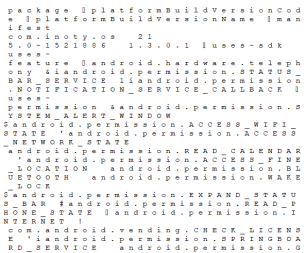
\includegraphics{fig1.png}
    \caption{A snippet of the AndroidManifest.xml file}
    \label{fig:my_label}
\end{figure}

\section{SPYWARE ANALYSIS}
In this section, I present observations and findings having analyzed the application’s Manifest file, source code, installation and execution on an Android device.
\subsection{A look at the AndroidManifest.xml file}
After performing an analysis of the manifest file (see Figure 1), several interesting points were found.
\begin{enumerate}
    \item Package name was identified as com.inoty.os with displayed version 1.3.0.1. The minSdkVersion for the app is 5.0 while the targetSdkVersion is 21. The package being used is net.suckga.inoty2.
    \item Permissions: the app requests several seemingly benign permissions, if considered on their own, such as Receive, System Alert Window, Access Fine Location, Access Network State, etc. However, when these permissions are considered together, they can be used for nefarious reasons. For example, these permissions can allow a malicious app to capture incoming messages and transmit them, along with the device’s location at the time, over a network. These and some other possibly harmful permissions are identified and briefly explained in Table 1.
    \item Activities, Services, Receivers and Content-Filters: Some of the more important ones will be examined in Section 4.5 below.
\end{enumerate}
\subsection{An Initial Look at the App’s Behavior}
Installing the .apk file was as simple as dragging and dropping it onto the emulator’sscreen. After the app was installed it was presented as an app named “Notify Ios” as shown in Figure 2a. When the app is launched, the first screen, depicted in Figure 2b offers several personalization options as well as a means of enabling the app. When the “Enable Notify Ios” option is selected, the user is presented with two services that could be turned on: Accessibility and Notifications. This is shown in Figure 2c. When the user chooses the Accessibility option, they are taken to the Accessibility Settings where they will be able to turn on “Notify Ios”. Once enabled, the user is told what privilege the app requires and asked for confirmation, as shown in Figure 2d. When the user chooses the Notifications option and enables the service, they are presented with a confirmation screen informing them of what access privileges the service will now have, as shown in Figure 3a. When the user enables both the accessibility and notification services, the app takes over the status bar (becomes the status bar) as shown in Figure 3b.
\subsection{Manipulations made while the app was active (sending texts, etc.)}
In order to test the functionality of the Notify Ios app, I enabled both the Accessibility and Notification services and then performed some activities to create notifications on the device. I sent text messages using the default Messages app and emails using the Gmail service. Figure 3c shows previously received notifications while Figure 3d shows an incoming notification from the Messages app.
\subsection{Network Analysis Process}
For us to determine whether the app was doing anything nefarious, I decided to capture the phone’s network traffic while the app was active. I discovered that every time the app was opened, it sent a GET request with some of the user’s private data to an IP address (204.11.56.48). I determined that this IP address was malicious and was based in the British Virgin Islands. Some information this app transmitted included the device’s model, the Operating System version, the phone’s IMEI number, the email address connected to the Google account on the device, the device’s MAC address, the current carrier, whether the device is rooted or not, the country location, etc., as shown in Figure 4. When both services were enabled, the app sent another GET request with the same information to the same IP address. However, this time it included a list of all the currently installed packages on the device, as shown in Figure 5.
\subsection{A look at the classes.jar file}
When the classes.jar file was opened with JD-GUI, I was presented with seven packages, each with several sub-packages which in turn contained several class files. The most interesting packages were found to be net.suckga.inoty2 and com.sweet.rangermob. The important classes and methods that were responsible for collecting and transmitting identifiable information about the device and user are highlighted below:
\newpage
\onecolumn
\begin{table}[]
\centering
\caption{Table 1. Permissions the Notify Ios Application Requests}
\label{tab:my-table}
\begin{tabular}{|l|l|}
\hline
\multicolumn{1}{|c|}{Permission} &
  \multicolumn{1}{c|}{Details} \\ \hline
android.permission.SYSTEM ALERT WINDOW &
  \begin{tabular}[c]{@{}l@{}}Allows an application to create windows that are shown on \\ top of all other apps.\end{tabular} \\ \hline
android.permission.ACCESS WIFI STATE &
  Allows applications to access information about Wi-Fi networks. \\ \hline
android.permission.ACCESS NETWORK STATE &
  Allows applications to access information about networks. \\ \hline
android.permission.READ CALENDAR &
  Allows an application to read the user’s calendar data. \\ \hline
android.permission.ACCESS FINE LOCATION &
  Allows an app to access the device’s precise location. \\ \hline
android.permission.BLUETOOTH &
  Allows applications to connect to paired Bluetooth devices. \\ \hline
android.permission.WAKE LOCK &
  \begin{tabular}[c]{@{}l@{}}Allows using PowerManager WakeLocks to keep processor from\\ sleeping or screen from dimming.\end{tabular} \\ \hline
android.permission.EXPAND STATUS BAR &
  Allows an application to expand or collapse the status bar. \\ \hline
android.permission.READ PHONE STATE &
  \begin{tabular}[c]{@{}l@{}}Allows read only access to the features of the phone, including \\ the phone number of the device, current cellular network \\ information, the status  of any ongoing calls, and a list of any \\ Phone Accounts registered on the device.\end{tabular} \\ \hline
android.permission.INTERNET &
  Allows applications to open network sockets. \\ \hline
android.permission.GET ACCOUNTS &
  Allows access to the list of accounts in the Accounts Service. \\ \hline
com.android.launcher.permission.INSTALL SHORTCUT &
  Allows an application to install a shortcut in Launcher. \\ \hline
android.permission.WRITE EXTERNAL STORAGE &
  Allows an application to write to external storage. \\ \hline
com.inoty.os.permission.C2D MESSAGE &
  \begin{tabular}[c]{@{}l@{}}Only this application can receive the messages and registration\\ result.\end{tabular} \\ \hline
com.google.android.c2dm.permission.RECEIVE &
  This app has permission to register and receive messages \\ \hline
\end{tabular}
\end{table}

\begin{figure}%
    \centering
    \subfloat[\centering label 1]{{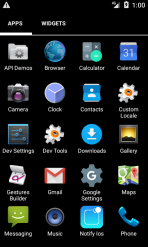
\includegraphics[width=3cm]{fig2a.png} }}%
    \qquad
    \subfloat[\centering label 2]{{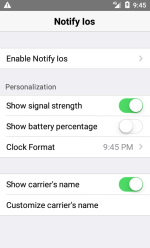
\includegraphics[width=3cm]{fig2b.png} }}%
    \qquad
    \subfloat[\centering label 2]{{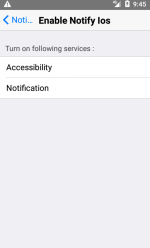
\includegraphics[width=3cm]{fig2c.png} }}%
    \qquad
    \subfloat[\centering label 2]{{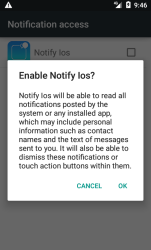
\includegraphics[width=3cm]{fig2d.png} }}%
    \caption{Figure 2. Screenshots of the Notify Ios app}%
    \label{fig:example}%
\end{figure}

\begin{figure}%
    \centering
    \subfloat[\centering label 1]{{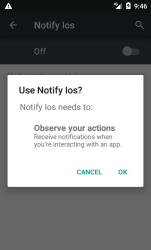
\includegraphics[width=3cm]{fig3a.png} }}%
    \qquad
    \subfloat[\centering label 2]{{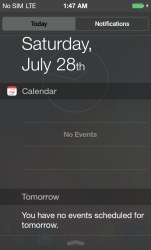
\includegraphics[width=3cm]{fig3b.png} }}%
    \qquad
    \subfloat[\centering label 2]{{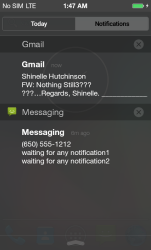
\includegraphics[width=3cm]{fig3c.png} }}%
    \qquad
    \subfloat[\centering label 2]{{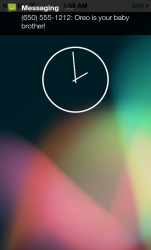
\includegraphics[width=3cm]{fig3d.png} }}%
    \caption{Figure 3. Screenshots of the Notify Ios app}%
    \label{fig:example}%
\end{figure}

\begin{figure}
    \centering
    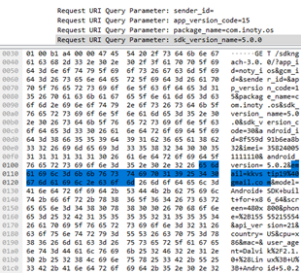
\includegraphics{fig4.png}
    \caption{Figure 4. Screenshot of PII data}
    \label{fig:my_label}
\end{figure}
\begin{figure}
    \centering
    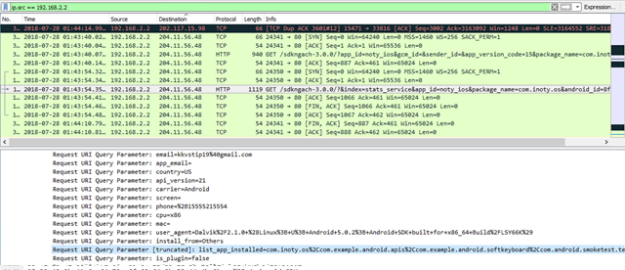
\includegraphics{fig5.png}
    \caption{List of all installed applications}
    \label{fig:my_label}
\end{figure}
\twocolumn
most interesting packages were found to be net.suckga.inoty2 and com.sweet.rangermob. The important classes and methods that were responsible for collecting and transmitting identifiable information about the device and user are highlighted below:

\begin{enumerate}
\item \emph{net.suckga.inoty2.preferences.PreferencesActivity}: It is the first class that runs when the app is launched by pressing its icon.
\item \emph{com.sweet.rangermob.helper.e.a(this.b)}: This method determines if there is an active internet connection. In such case, the com.sweet.rangermob.a() method is started.
\item \emph{com.sweet.rangermob.a()}: This method collects identifying information about the device and user which is subsequently transmitted to the rogue IP address. This information is stored in a variable called localArrayList.
\item \emph{RootUtil.a()}: It looks for superuser access (determines if phone is rooted).
If the device is rooted, collects several other pieces of information, including whether the device has Google Play Store installed, whether there is an active device admin, etc., and adds this information to the localArrayList variable.
\item \emph{paramAnonymousVarArgs \ URLEncodedUtils.format (localArrayList, “utf-8”)}: converts the localArrayList to a URL.
\item \emph{j.a() + paramAnonymousVarArgs}: This builds the website’s URL and concatenates it with the Encoded URL from localArrayList with help from the com.sweet.rangermob.helper.c class. 
\item \emph{com.sweet.rangermob.helper.c}: This class contains variables used to build the HTTP GET request and the domain website.
\item \emph{paramAnonymousVarArgs=com.sweet.rangermob.helper.b.b(j.a() + paramAnonymousVarArgs)}: This passes the completed URL string to be created in the HTTP GET request.
\item Within the com.sweet.rangermob.xser.RangerSer class, there is a method that handles collecting and sending the device and user information, in addition to a list of all the installed packages on the device, to the rogue IP address. This method closely resembles the one that runs every time the app is opened.
\end{enumerate}
\subsection{Interesting Findings}
In an attempt to determine whether or not this app would be flagged by Google’s Play Protect service, I attempted to install the Notify Ios app on a physical Samsung Galaxy S5 device running Android 6.0. The device was set to allow installation of apps from third parties. I performed this installation on three separate occasions because the Play Protect service detects malware using machine learning techniques. This will show us whether those techniques are efficient against such malware as Notify Ios.
\subsubsection{July 28th, 2021}
The .apk file was copied onto the device
and was able to successfully install the app.
When Play Protect scanned all the apps on
the device, none were flagged as suspicious.
\newpage


\subsubsection{Oct 12th, 2021}
The .apk file was again copied onto the device and attempted to install the app. However, the Play Protect service immediately flagged the app as suspicious, as shown in Figure 6.
\subsubsection{Oct 14th, 2021}
One last attempt to install the app on the device, however this time there was no Play Protect warning and the app simply did not install, as shown in Figure 7. From these occurrences, I believe that the Play Protect service learned from my first installation of the Notify Ios app and now is able to block any installation of the app on devices.
\begin{figure}
    \centering
    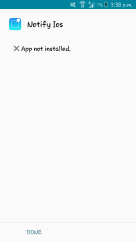
\includegraphics{fig7.png}
    \caption{Screenshot of Noty Ios app refusing to be installed.}
    \label{fig:my_label}
\end{figure}
\begin{figure}
    \centering
    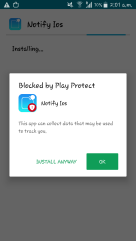
\includegraphics{fig6.png}
    \caption{Screenshot of Play Protect service blocking the installation of Noty Ios}
    \label{fig:my_label}
\end{figure}
\section{GUIDELINES FOR MOBILE APPLICATION ANALYSIS}
\begin{enumerate}
    \item Static Analysis: Be sure to investigate the source code and app manifest files, looking for suspicious implementations and unnecessary permission requests that do not fit the described use of the app. This step can be extremely cumbersome should the app developer obfuscate the source code, specifically class, method and variable names. 
    \item Dynamic Analysis: Static analysis alone tends to be insufficient for determining exactly what an app is doing. Once you have an idea of what the app is doing from the static analysis, be sure to install the app on a clean device and run it. This way, you can interact with the app, manipulate various features and note its effects on the device.
    \item Network Analysis: Many apps, especially spyware apps, use network features and chances are if you suspect the app is doing something nefarious after doing static and dynamic analysis, the app may be communicating with a malicious, remote server. You should make network analysis a step during your dynamic analysis. Using a network sniffer like Wireshark could allow you to ascertain what communications the app is doing while it’s running on a device. This includes determining what information the app is transmitting and to whom that data is going to.
\end{enumerate}
After performing each of these, you should
have a fairly comprehensive understanding
of what the app does and how its features
are implemented.
\section{CONCLUSION}
Android smartphones are widely used, and
their users require protection from nefarious
individuals set on obtaining these users’ PII.
Unfortunately, it is possible for some apps
to covertly collect user’s PII and transmitted
that data to unauthorized persons.
\par After my analysis of the Notify Ios malicious app, I determined that various pieces  of users’ PII were being transmitted to an unauthorized location. I also combed through the source code to identify exactly how this was being accomplished and quickly found that the app developer relied heavily on obfuscation of their code to mask their ill intent. I also tested the capacity of Google’s Play Protect service to detect this malicious app and was able to prove that the service initially failed to detect the app. However, it was able to learn and flag the app on subsequent installations.
\par For future work, I intend to develop my own malicious spyware app in an attempt to successfully avoid detection by the Play Protect service. In doing so, I aim to identify certain malicious characteristics the service is still incapable of detecting as well as specific vulnerabilities the service is still susceptible to.


\begin{thebibliography}{00}
\bibitem{1} 
Abualola, H., Alhawai, H., Kadadha, M., Otrok, H., \& Mourad, A. (2016). An android-based trojan spyware to study the notificationlistener service vulnerability. Procedia Computer Science, 83, 465 - 471. Retrieved from {\fontfamily{qcr}\selectfont \url{http://www.sciencedirect.com/science/article/pii/S1877050916302435}} (The 7th International Conference on Ambient Systems, Networks and Technologies (ANT 2016) / The 6th International Conference on Sustainable Energy Information Technology (SEIT-2016) / Affiliated Workshops) doi: https://doi.org/10.1016/j.procs.2016.04.210
\bibitem{2}  
Ashishb. (2018). ashishb/android-malware. Retrieved from {\fontfamily{qcr}\selectfont \url{https://github.com/ashishb/ android-malware/tree/master/Android.Spy.277.origin}}
\bibitem{3}
Google detects android spyware that spies on whatsapp, skype calls. (2017, Nov). The Hacker News. Retrieved from {\fontfamily{qcr}\selectfont \url{https://thehackernews.com/2017/11/android-spying-app.html?}}
\bibitem{4}
Google play protect. (2018). Android. Retrieved from {\fontfamily{qcr}\selectfont \url{https://www.android.com/play-protect/}}
\bibitem{5}
Kaur, P., \& Sharma, S. (2015). Spyware detection in android using hybridization of description analysis, permission mapping and interface analysis. Procedia Computer Science
\bibitem{6}
Khandelwal, S. (2017, Nov). Fake whatsapp on google play store downloaded by over 1 million android users. The Hacker News. Retrieved from {\fontfamily{qcr}\selectfont \url{https://thehackernews.com/2017/11/fake-whatsapp-android.html?utm\_source=feedburner\&utm\_medium=feed&utm\_campaign=ewlineFeed:TheHackersNews(TheHackersNews-SecurityBlog)\&\_m=3n.009a.1616.pv0ao08grr.z3r}}
\bibitem{7}
Mahindru, A., \& Singh, P. (2017). Dynamic permissions based android malware detection using machine learning techniques. In Proceedings of the 10th innovations in software engineering conference (pp. 202–210).
\bibitem{8}
Malik, J., \& Kaushal, R. (2016). Credroid: Android malware detection by network traffic analysis. In Proceedings of the 1st acm workshop on privacy-aware mobile computing (pp. 28–36).
\bibitem{9}
Mobile operating system market share worldwide. (2018, Oct). Retrieved from http://gs.statcounter.com/os-market-share/mobile/worldwide#monthly-201708-201709-bar
\bibitem{10}
Mobile operating system market share worldwide. (2018, Oct). Retrieved from {\fontfamily{qcr}\selectfont \url{http://gs.statcounter.com/os-market-share/mobile/worldwide#monthly-201708-201709-bar}}
\bibitem{11}
Rathi, D., \& Jindal, R. (2018). Droidmark: A tool for android malware detection using taint analysis and bayesian network. arXiv preprint arXiv:1805.06620 .
\bibitem{12}
Ren, J., Rao, A., Lindorfer, M., Legout, A., \& Choffnes, D. (2016). Recon: Revealing and controlling pii leaks in mobile network traffic. In Proceedings of the 14th annual international conference on mobile systems, applications, and services (pp. 361–374).
\bibitem{13}
Saracino, A., Sgandurra, D., Dini, G., \& Martinelli, F. (2018). Madam: Effective and efficient behavior-based android malware detection and prevention. IEEE Transactions on Dependable and Secure Computing, 15 (1), 83–97.
\bibitem{14} 
Wang, J., Li, B., \& Zeng, Y. (2017). Xgboost-based android malware detection. In Computational intelligence and security (cis), 2017 13th international conference on (pp. 268–272).

\end{thebibliography}
\end{document}
